\subsection{初段ミューオントリガーにおけるエレクトロニクス}
初段ミューオントリガーでは、ATLAS 検出器から送られてくる情報に対して SectorLogic、MUCTPI、L1Topo、CTP という電子回路を経てトリガーが発行される。
以下では各エレクトロニクスについて説明する。

\subsubsection{Amplifier Shaper Discriminator (ASD) ボード}
Amplifier Shaper Discriminator (ASD) ボードは TGC のワイヤーとストリップからアナログ信号を受け取り、デジタル信号への変換を行う。
ASD ボード上の ASD において TGC からのアナログ信号を増幅・整形し、 閾値電圧を超えた信号のみ LVDS 信号として出力される。1 枚の ASD ボードは 4 つの ASD ASIC を搭載しており、ASD ASIC は 4 つの信号の受信・処理を行う。そのため、同時に 16 チャンネルの信号を処理することが可能である。

\subsubsection{Patch-Panel ASIC (PP ASIC)}
Patch-Panel ASIC は ASD からワイヤーとストリップそれぞれの LVDS 信号を受け取り、タイミングの調整を行うことで、同じ陽子衝突由来の信号を同時に次の SLB ASIC に送る。陽子衝突が起きてからミューオンが検出器に到達する時間や、ケーブルの長さの違いにより、信号のタイミングが各チャンネルごとに異なるため、PP ASIC を用いてタイミングの調整を行う。

\subsubsection{Slave Board ASIC (SLB ASIC)}
Slave Board ASIC は読み出しとトリガー判定の 2 種類の処理を行う。
トリガー判定で行う処理としては、各チャンネルの情報を用いてコインシデンスを取ることである。
TGC Triplet (M1 ステーション) ではワイヤーの場合は 3 層中 2 層にヒットがあることを要求し、ストリップの場合は 2 層中 1 層にヒットがあることを要求する。
2 つの TGC Doublet (M2、M3 ステーション) では、各ステーションから信号を受け取りワイヤーとストリップで独立に 4 層中 3 層以上にヒットがあることを要求する。 これらのコインシデンス結果はLVDS 信号で後段の High PT ボードに送る。

\subsubsection{High PT (HPT) ボード}
High PT ボードは、M1 の SLB と M2,M3 の SLB からのコインシデンス結果を受け取り、 M1,M2,M3 の 3つのステーション間のコインシデンスを行う。M1 と M3 の位置情報から ($\Delta R$, $\Delta \phi$) を計算し、次の Sector Logic に送る。Sector Logic にはボードごとに、位置情報 $R$ と $\phi$ 、位置の差の情報 $\Delta R$ と $\Delta \phi$ を G-Link 通信を用いて送信する。データ通信速度の制限により、1 つの HPT ASIC から最大 2 候補を選んで送信している。

\subsubsection{New Sector Logic (NSL)}
New Sector Logic では TGC-BW とトロイド磁石の内側にある検出器の情報を統合してトリガー判定を行う。
TGC-BW の HPT ボードからは、ミューオン候補の情報が G-Link 規格で送られてくる。
RPC BIS78、Tile カロリメータ、 TGC-EI からは、検出器におけるヒット情報が送られてくる。
NSW からは通過したミューオンの飛跡情報が送られてくる。
NSL はこれらの情報をもとにトリガー判定を行い、トリガー判定の結果を MUCTPI に送信する。

NSL ボードでは、 HPT ボードから受け取った TGC BW の位置情報 $R$ と $\phi$ 、位置の差の情報 $\Delta R$ と $\Delta \phi$ を用いて $p_T$ の判定を行う。各 ($R$, $\phi$) からミューオンのヒット位置を表す RoI を決定し、($\Delta R$, $\Delta \phi$) から NSL 上に実装されている Coincidence Window を用いて $p_T$ に変換する。



%\begin{figure}
    %\centering
%    \begin{tabular}{cc}
%    \begin{minipage}[b]{0.45\hsize}
%        %\centering
%        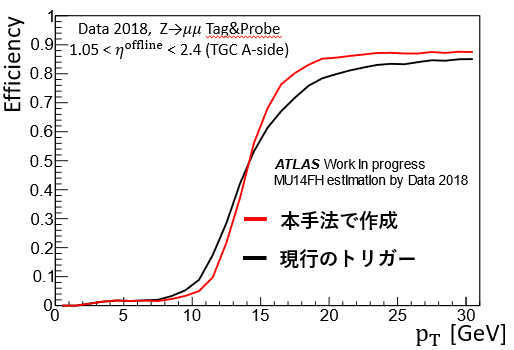
\includegraphics[clip, width=7cm]{fig/4/hikaku_v05_v06.png}
%        %\vspace{5pt}
%        \subcaption{}
%        \label{fig:v05v06}
%    \end{minipage}&
%    %\hfill
%    \begin{minipage}[b]{0.45\hsize}
%        %\centering
%        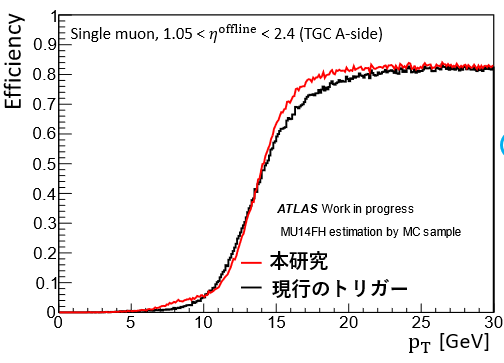
\includegraphics[clip, width=7cm]{fig/4/hikaku_v05_v07.png}
%        %\vspace{5pt}
%        \subcaption{}
%        \label{fig:v05v07}
%    \end{minipage}
%    \end{tabular}
%    \caption{ある閾値におけるTurn-on curveの現行のトリガーとの比較。(a):実際のデータを用いてトレーニングを行った機械学習から作成したCWとの比較。(b): シミュレーションデータを用いてトレーニングを行った機械学習から作成したCWとの比較。}
%    \label{}
%\end{figure}

%\begin{figure}[tb]
%  \centering
%  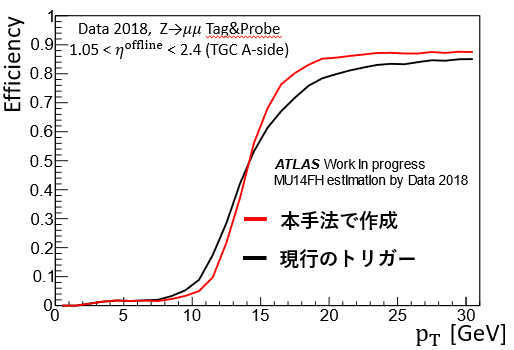
\includegraphics[clip, width=12cm]{fig/4/hikaku_v05_v06.png}
%  \caption{v05v06}
%  \label{fig:v05v06}
%\end{figure}

%\begin{figure}[tb]
%  \centering
%  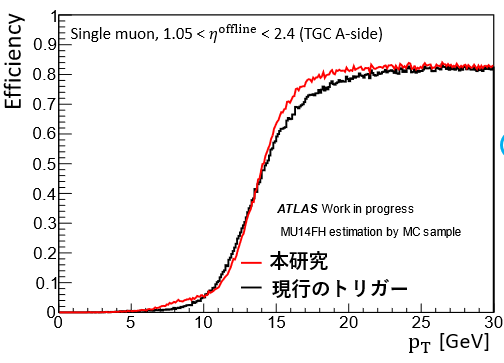
\includegraphics[clip, width=12cm]{fig/4/hikaku_v05_v07.png}
%  \caption{v05v07}
%  \label{fig:v05v07}
%\end{figure}





